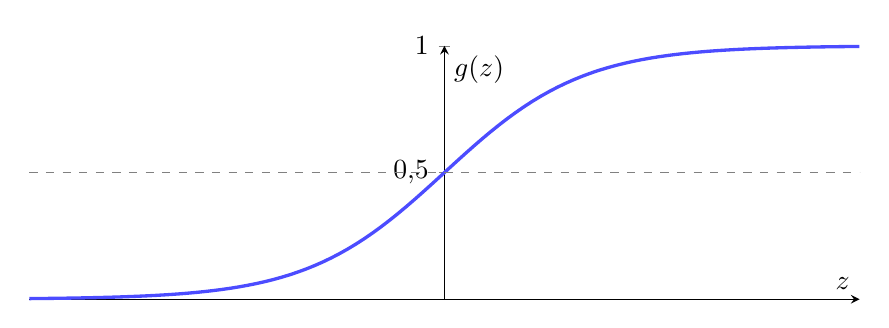
\begin{tikzpicture}
    \begin{axis}[
        width=\textwidth,
        height=4.8cm,
        xmin=-6, xmax=6,
        ymin=0, ymax=1,
        axis lines=middle,
        xlabel={$z$},
        ylabel={$g(z)$},
        xtick={0},
        ytick={0,0.5,1},
        yticklabels={$0$,$0{,}5$,$1$},
        clip=false
    ]
        \addplot[
            very thick,
            blue!70,
            domain=-6:6,
            samples=100
        ] {1/(1+exp(-x))};

        \addplot[
            dashed,
            gray,
            domain=-6:6,
            samples=2
        ] {0.5};
    \end{axis}
\end{tikzpicture}
